
\documentclass[12pt]{article}
\usepackage[top=1in, bottom=1in, left=1in, right=1in]{geometry} % see geometry.pdf on how to lay out the page. There's lots.
\usepackage{graphicx}
\geometry{letterpaper} % or letter or a5paper or ... etc
% \geometry{landscape} % rotated page geometry
\usepackage{hyperref}

% See the ``Article customise'' template for come common customisations

\title{MADAI Workbench 1.8.0 Tutorial: \\A Supplement to the ParaView Tutorial}
\author{Cory Quammen}
\date{} % delete this line to display the current date

\newcommand{\filter}[1]{\textbf{#1}}
\newcommand{\filterinstance}[1]{\texttt{#1}}
\newcommand{\menu}[1]{\textbf{#1}}
\newcommand{\representation}[1]{\texttt{#1}}
\newcommand{\file}[1]{\texttt{#1}}
\newcommand{\setting}[1]{\textbf{#1}}
\newcommand{\field}[1]{\texttt{#1}}

%%% BEGIN DOCUMENT
\begin{document}


\maketitle
\tableofcontents

\section{Introduction}

The MADAI Workbench is a visualization program based on ParaView. It uses ParaView's plugin-mechanism to provide features over and above what ParaView provides in addition to all the great features already in ParaView.

The first question you must answer when attempting to use a visualization tool is how to get the your data into the visualization program. The first half of this tutorial starts with some examples of converting example data files into a format that can be imported by the MADAI Workbench. 

The second half of this tutorial will walk you through using several of the extensions that the MADAI Workbench provides. These features are not available in a plain installation of ParaView.

The content of this tutorial assumes that you have gone through the ParaView Tutorial for version 3.98 or higher of ParaView. You also need the tutorial data in the ZIP file \file{MADAIWorkbenchTutorial.zip}.

\section{Importing Data}

The MADAI Workbench can import many different file types. We first start with a relatively simple conversion of an example text file containing data from a simulation into a VTK (Visualization Toolkit) file that the MADAI Workbench can load. Next we convert two different kinds of OSCAR (Open Standard Codes and Routines) files into XDMF files that the MADAI Workbench can read.

\subsection{Importing a Text File}

It is often the case that simulation codes produce output files in a custom format that no other programs can read. In some cases, however, the output format file may be modified slightly to become a file that the MADAI Workbench can read. We will be loading ASCII files written by a particular program that has five data points per line separated by spaces with no header. We’re going to edit this file (make a copy first) to turn it into a VTK file. This file format is described in the \href{http://www.vtk.org/VTK/img/file-formats.pdf}{VTK File Formats PDF}.

Copy the file \file{AR.spec} to \file{AR.vtk}. Open \file{AR.spec} in your favorite text editor and paste the following text into the beginning of the file. Do not include the portions of the line following \verb+//+. Make sure to get the correct number of spaces in each line. Note the space between the \verb+#+ and \verb+vtk+ in the first line.

\begin{verbatim}
# vtk DataFile Version 2.0   // File-format indicator string (“magic cookie”)
Converted Jonathan Lees file // This comment line  must be present
ASCII
DATASET STRUCTURED_POINTS 
DIMENSIONS 7461 4096 1       // Tells the number of points in X, Y, and Z 
SPACING 1 1 0                // Computed based on number of points and X,Y extent
ORIGIN 0 0 0                 // Centered around (0,0) in X and Y
POINT_DATA 30560256          // 7461x4096x1 total data values
SCALARS AR float 1           // One scalar per value. Name based on file name (AR)
LOOKUP_TABLE default         // Use the default color map
\end{verbatim}

After you save the file with your modifications, load it in the MADAI Workbench. It will probably take a long time to parse and load the ASCII file. To make future operations faster, you can save the data as a binary file that will be loaded later. To do this, select \menu{File} $\rightarrow$ \menu{Save Data} and then change the \setting{Files of type} menu to ``VTK ImageData Files (*.vti)''. Give the file the name \file{AR.vti} and click \setting{OK}. Make sure \setting{Compressor Type} is set to None. Now, when you load \file{AR.vti}, it will read in much faster.

Now do the same modifications to the files \file{MTM.FVMAT} and \file{MTM.spec} files to produce \file{FV.vti} and \file{M\_small.vti}.

\subsubsection{Combining Different Data Fields}

The files you produced in the previous section each contain a single scalar data field. For certain visualization techniques, the separate scalar data fields must be combined into a single dataset. The \filter{Append Attributes} filter makes it possible to combine the different data sets.

Load the files \file{AR.vti}, \file{FV.vti}, and \file{M\_small.vtk}. Select all three by clicking the first file in the pipeline browser, then press the shift key and click the last file in the pipeline browser. Next, select \menu{Filters} $\rightarrow$ \menu{Alphabetical} $\rightarrow$ \menu{Append Attributes}. This file creates a new object that has all three data sets included in it.

Click on \filterinstance{AppendAttributes1} and choose \menu{File} $\rightarrow$ \menu{Save Data}. Save this file as a VTI binary file. In the future, you can load just this file and have all three data fields loaded. This is more convenient than having to load each data field file separately.

\subsubsection{Visualizing Two Data Fields in 2D}

With the \filterinstance{AppendAttributes1} still selected, select \filter{Filters} $\rightarrow$ \filter{Alphabetical} $\rightarrow$ \filter{Extract Surface}. Next, select \filter{Filters} $\rightarrow$ \filter{Alphabetical} $\rightarrow$ \filter{Warp Scalar}. SETTINGS. Choose the \field{AR} for \setting{Coloring}. Now, add a \menu{Filters} $\rightarrow$ \menu{Alphabetical} $\rightarrow$ \menu{Contour} filter to \filterinstance{WarpScalar1}. Set the contour value(s) to XXX and the data field to \field{FV}.

Figure XXX shows the three data fields with different display channels (height surface, color scale, and isocontour lines).

\subsection{Converting OSCAR Files}

People in the high-energy physics community often produce OSCAR (Open Standard Codes and Routines) files from their simulation codes. To get these data into the MADAI Workbench, a couple external conversion utilities are available to turn OSCAR files into XDMF files that can be read by the MADAI Workbench. Two different converters are available, one that converts OSCAR1997a files and one that converts OSCAR2008H files. In this section, we will see how to use the converters to create files that can be visualized in the MADAI Workbench.

\subsection{Converting OSCAR1997A Files}

Run the following commands

\begin{verbatim}
> cd OSCARData/1997A
> oscar1997a_to_xdmf-1.1.2 -i AuAu_s200_b2_t100_1ev-1.f19 \
   -o AuAu_s200_b2_t100_1ev-1
\end{verbatim}

The \texttt{-i} option gives the input name of the OSCAR file to convert while the \texttt{-o} option gives the prefix of the output file names. The converter produces two files, one with the extension \texttt{.h5} and one with the extension \texttt{.xmf}. When you run this command, you should see two new files created in your working directory, \texttt{AuAu\_s200\_b2\_t100\_1ev-1.xmf} and \texttt{AuAu\_s200\_b2\_t100\_1ev-1.h5}.

Now open the \texttt{AuAu\_s200\_b2\_t100\_1ev-1.xmf} file in the MADAI Workbench. You should see XXX.

There are additional options available in this OSCAR converter program. Run

\begin{verbatim}
> oscar1997a_to_xdmf-1.1.2 --help
\end{verbatim}
to see additional options.

\subsection{Converting OSCAR2008H Files}

Run the following commands

\begin{verbatim}
> cd OSCARData/2008H
> oscar2008h_to_xdmf-1.1.2 -i e160_b7_3e0_coarse_truncated.dat \
   -o e160_b7_3e0_coarse_truncated
\end{verbatim}

As with the conversion of the OSCAR1997A files, you will see two new files, \\ \texttt{e160\_b7\_3e0\_coarse\_truncated.xmf} and \texttt{e160\_b7\_3e0\_coarse\_truncated.h5}.

Now open the \texttt{e160\_b7\_3e0\_coarse\_truncated.xmf} file 

There are additional options available in this OSCAR converter program. Run

\begin{verbatim}
> oscar2008h_to_xdmf-1.1.2 --help
\end{verbatim}
to see additional options.

\section{MADAI Workbench Features}

\subsection{Threshold Points Filter}

One type of data you may want to view is point data, especially if your work involves simulating particle systems. You may want to threshold a point set to show only points that have a variable value within some range. There is a problem with the \filter{Threshold} filter provided by ParaView when you try to do this. This filter operates on cells in a dataset. Cells, such as triangle or tetrahedra, are elements that either have a surface area or volume. This is a problem when your dataset consists of points with no associated cells. This can show up in strange ways when you have applied a \filter{Threshold} filter to your dataset, but no filtering appears to have been done.

\begin{figure}[htbp]
   \centering
   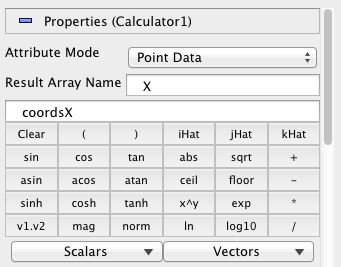
\includegraphics[scale=.5]{images/ThresholdPointsFilterCalculator.png} % requires the graphicx package
   \caption{Creating a point scalar field for the point data.}
   \label{fig:ThresholdPointsFilterCalculator}
\end{figure}

To see that this is the case, create a point source by selecting \menu{Sources} $\rightarrow$ \menu {Point Source}. Change the \setting{Number of Points} to 1000 and \setting{Radius} to 1. Next, create a \filter{Calculator} filter by selecting \menu{Filters} $\rightarrow$ \menu{Alphabetical} $\rightarrow$ \menu{Calculator}. Set the \setting{Result Array Name} to ``X'' and enter ``coordsX'' in the text field above the calculator buttons (you can also click on the \menu{Scalars} menu and select \menu{coordsX}). Figure \ref{fig:ThresholdPointsFilterCalculator} shows the settings for the calculator. This creates a point scalar field that has the same value as the $x$-coordinates of the points.

Now apply the \filter{Threshold} filter (\menu{Filters} $\rightarrow$ \menu{Alphabetical} $\rightarrow$ \menu{Threshold}). Select ``X'' from the \setting{Scalars} menu and uncheck the \setting{All Scalars} checkbox and then click \setting{Apply}. You should still see all the original points in the 3D View. Next, change the \setting{Maximum} value to 0.2. Again, all the original points are displayed, indicating that thresholding did not work. Now delete the \filterinstance{Threshold1} filter.

Now we will perform thresholding that works for point data sets. Select the \filterinstance{Calculator1} filter in the Pipeline Browser again and this time create a \filter{Threshold Points} filter (\menu{Filters} $\rightarrow$ \menu{Alphabetical} $\rightarrow$ \menu{Threshold Points}). Select ``X'' as the scalars and change the right value of the \setting{Threshold Range} to 0.2. This time, the points will be filtered such that points with the X value (and $x$-coordinate) above 0.2 are removed from the point set, as shown in Figure \ref{fig:ThresholdPointsFilter}.

\begin{figure}[htbp]
   \centering
   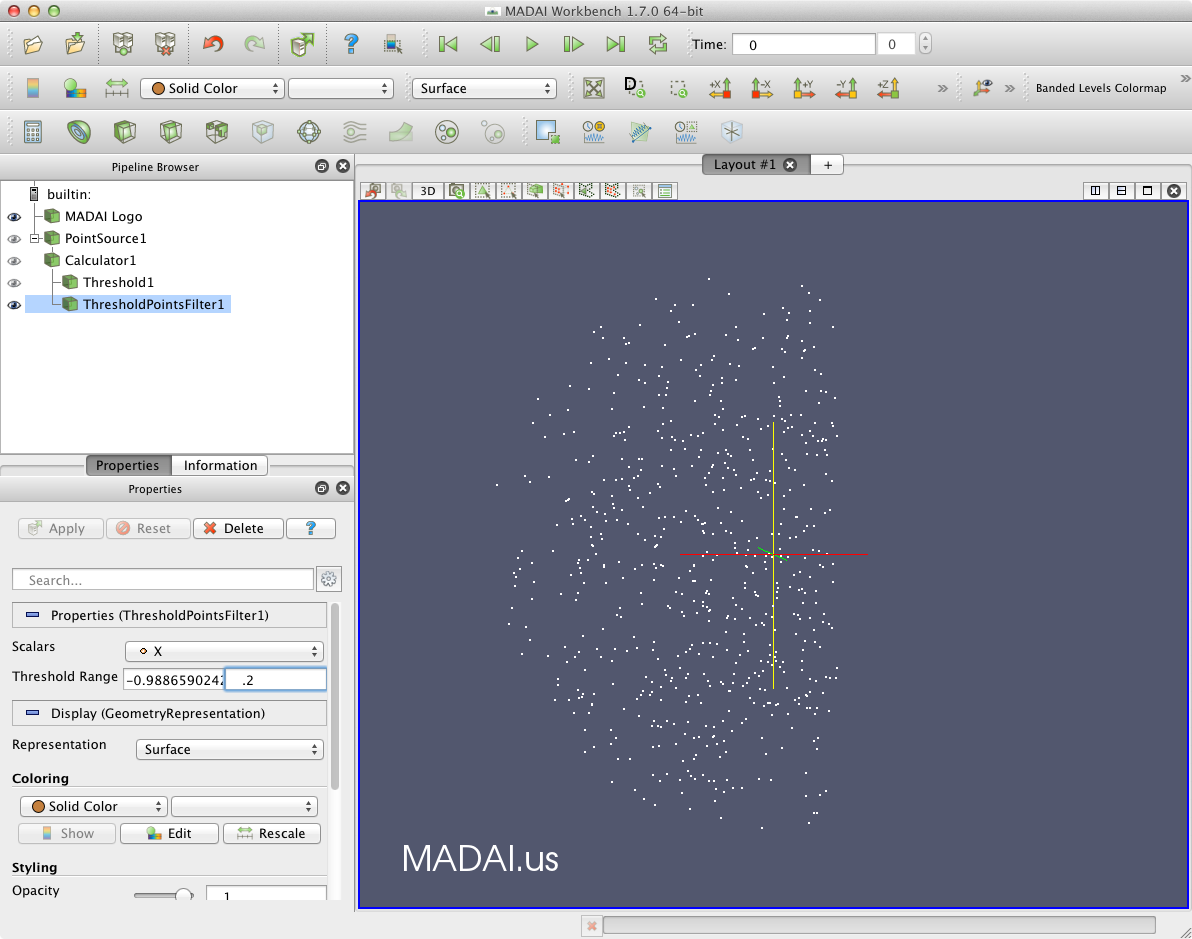
\includegraphics[scale=.25]{images/ThresholdPointsFilter.png} % requires the graphicx package
   \caption{Results of the \filter{Threshold Points} filter.}
   \label{fig:ThresholdPointsFilter}
\end{figure}

\subsection{Binning Filter}

When you have a large number of points, it may be difficult to estimate certain quantities such as local density of points because of \emph{overplotting}. Overplotting occurs when there are fewer pixels than points to display; more than one point will map to one pixel in the display, and you will see only the nearest point.

In cases of overplotting, you can instead compute an intermediate dataset that stores density information by using the \filter{Binning} filter. The \filter{Binning} filter provides a fast way to create a regular 2D or 3D grid representing density from a point set.

If you have completed the exercise from the previous section, delete the and \filterinstance{ThresholdPoints1} filters from the pipeline by right-clicking them and choosing the menu item \menu{Delete}. Now click on the \filterinstance{PointSource1} source and change the \setting{Number of Points} to 100,000. Now apply a \filter{Binning} filter to it (\menu{Filters} $\rightarrow$ \menu{Alphabetical} $\rightarrow$ \menu{Binning} filter). The default settings are fine. Click \setting{Apply}. Now set the representation to \representation{Slice} and set the \setting{Slice Direction} to XY Plane. Move the \setting{Slice} to the middle of the range. In the \setting{Coloring} section, choose the \field{NumberDensity} point field in the popup menu and click the \setting{Rescale} button. You should see an image similar to Figure \ref{fig:BinningFilter}.

\begin{figure}[htbp]
   \centering
   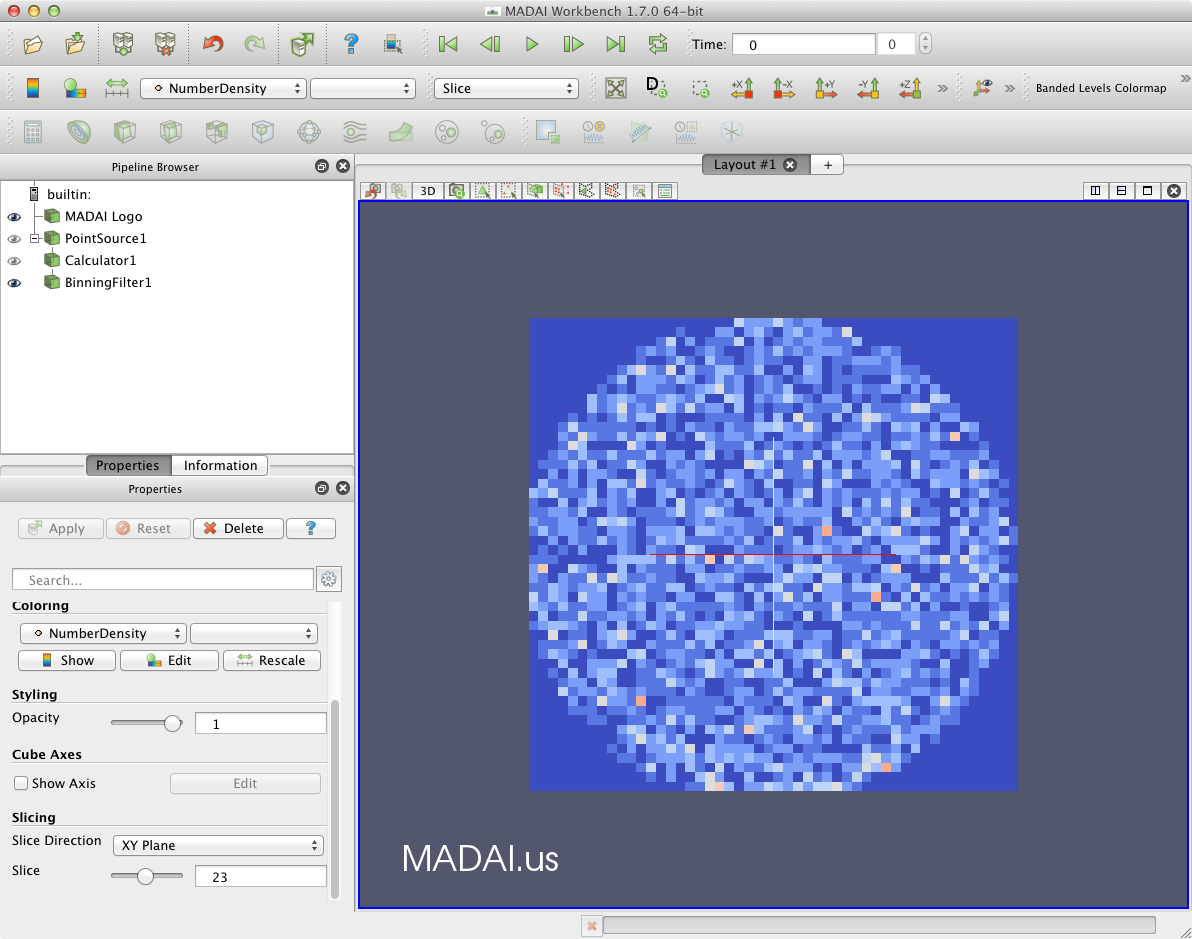
\includegraphics[scale=.25]{images/BinningFilter.png} % requires the graphicx package
   \caption{Results of the \filter{Binning} filter.}
   \label{fig:BinningFilter}
\end{figure}

The \field{NumberDensity} field gives the number of points that fall within each grid cell. In addition to the \field{NumberDensity} field, the binning filter also sums up each point data field. Change the point data field in the \setting{Coloring} section to \field{X\_Density}. The value of each grid point in this filter's output is the sum of all the \field{X} values of the points that fall within the cell (see Figure \ref{fig:BinningFilterXDensity}).

\begin{figure}[htbp]
   \centering
   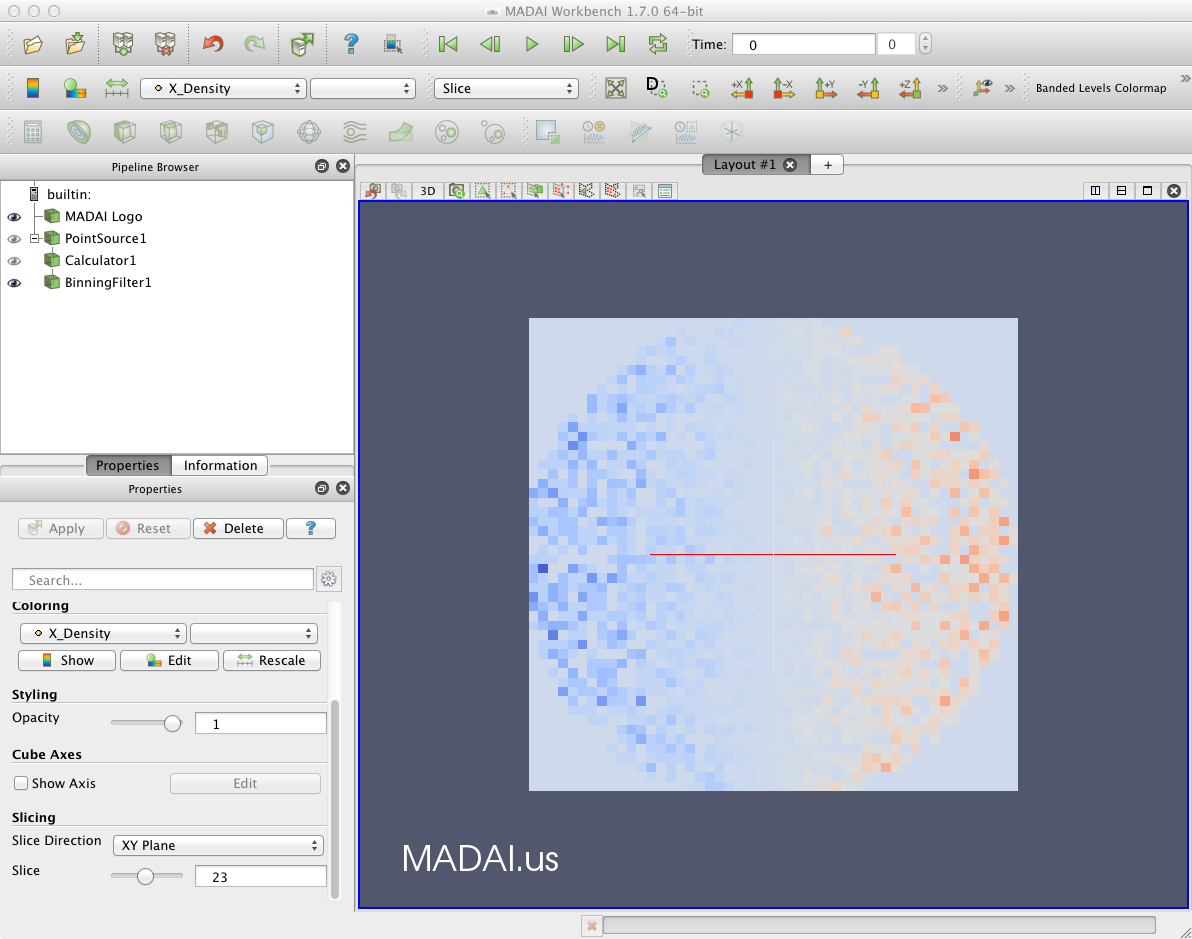
\includegraphics[scale=.25]{images/BinningFilter_XDensity.png} % requires the graphicx package
   \caption{The \texttt{X\_Density} field computed by the \textbf{Binning} filter from the \texttt{X} field.}
   \label{fig:BinningFilterXDensity}
\end{figure}

To get the average density of the points in the grid cell, you can divide the \field{X\_Density} field by the \field{NumberDensity} field. To do this, apply a \filter{Calculator} filter to \filterinstance{BinningFilter1}, set the \setting{Result Array Name} to \field{AverageX}, and set the text field to ``X\_Density / NumberDensity'' (without the quotation marks).  Choose the \field{AverageX} field in the \setting{Coloring} section and click the \setting{Rescale} button. The image will look largely the same as Figure \ref{fig:BinningFilterXDensity}. The main difference is that the range of the \field{AverageX} is now close to [-1,1]. You can confirm this by clicking on \textbf{Information} tab. Under \setting{Data Arrays}, you will see a table showing field names, field data types, and the numeric ranges of the fields. Look at the table row for field \field{AverageX}. It is slightly smaller than the range [-1,1]. Because this is in a sense the average $x$-coordinate value from the points in each bin and the points were sampled from a sphere with radius 1, this range makes sense. 

\subsection{Gaussian Scalar Splatter Filter}

Whereas the \filter{Binning} filter computes discrete summation of points within a grid cell, the \filter{Gaussian Scalar Splatter} filter computes smoother density fields by spreading the values associated with each point according to an isotropic 3D Gaussian ``splat'' function whose integrated energy is 1. The 3D Gaussian splat's size is controlled by the standard deviation parameter of the Gaussian and is specified in the units of the space in which the data is embedded (e.g., meters). The splat size determines how far the influence of each point reaches and how smooth the resulting scalar field.

The \filter{Gaussian Scalar Splatter} operates on each point in the input dataset. For each input point, the splat is centered at the point. The integrated portion of the splat that intersects a grid cell in the output is computed and added to the value at the cell. After each point is processed, each cell in the output has a number density similar in concept to the number density field produced by the \filter{Binning} filter. In fact, this filter produces the same results as the binning filter as the size of the splat approaches 0. Each point data field \field{F} is multiplied by this integrated value and added to a new data field called \field{F\_Density}. An important feature of this filter is that if you integrate a dataset field produced by the filter and integrate the dataset field input to this filter, the answer is the same (within some tolerance). This is true no matter the resolution of the output dataset.

Click on the \filterinstance{PointSource1} filter and change the \setting{Number of Points} to 1000. If you do not change this number to 1000, it will take too long to compute.

Next, add a \filter{Gaussian Scalar Splatter} filter (\menu{Filters} $\rightarrow$ \menu{MADAI} $\rightarrow$ \menu{Gaussian Scalar Splatter}) to \filterinstance{Calculator1}. Leave the \textbf{Standard Deviation} setting at 0.1, but change the \textbf{Sample Dimensions} to 25 25 25. (\emph{\textbf{WARNING}}: if you don't change the \textbf{Sample Dimensions} to 25 25 25, you will be wait a \emph{very} long time for the filter to finish.) Click the \setting{Apply} button. Next, change the representation to \representation{Volume}, color the data by \field{NumberDensity}, and click the \setting{Rescale} button. You should see an image similar to the left side of Figure \ref{fig:GaussianScalarSplatter1}.

\begin{figure}[htbp]
   \centering
   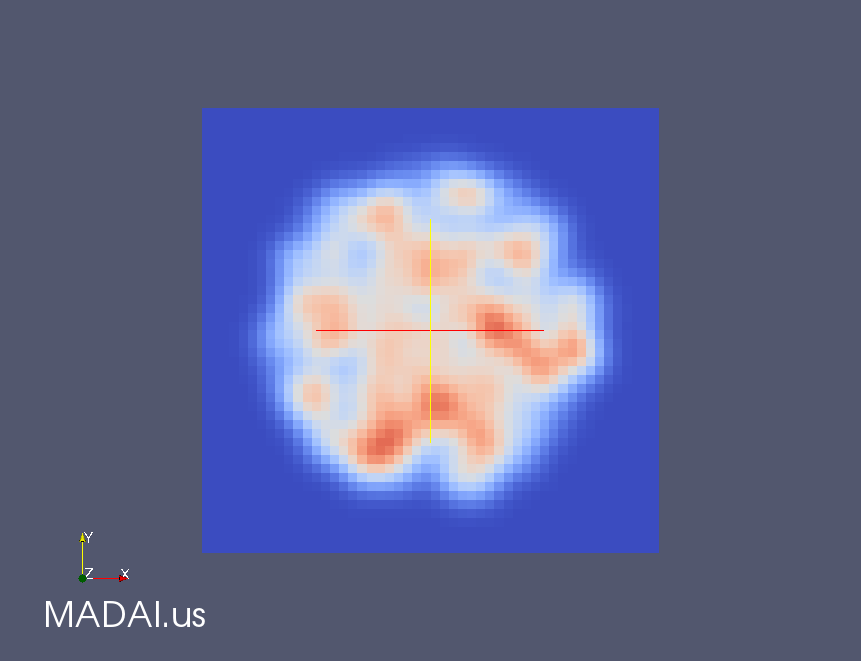
\includegraphics[scale=.22]{images/GaussianScalarSplatterPoint1.png}
   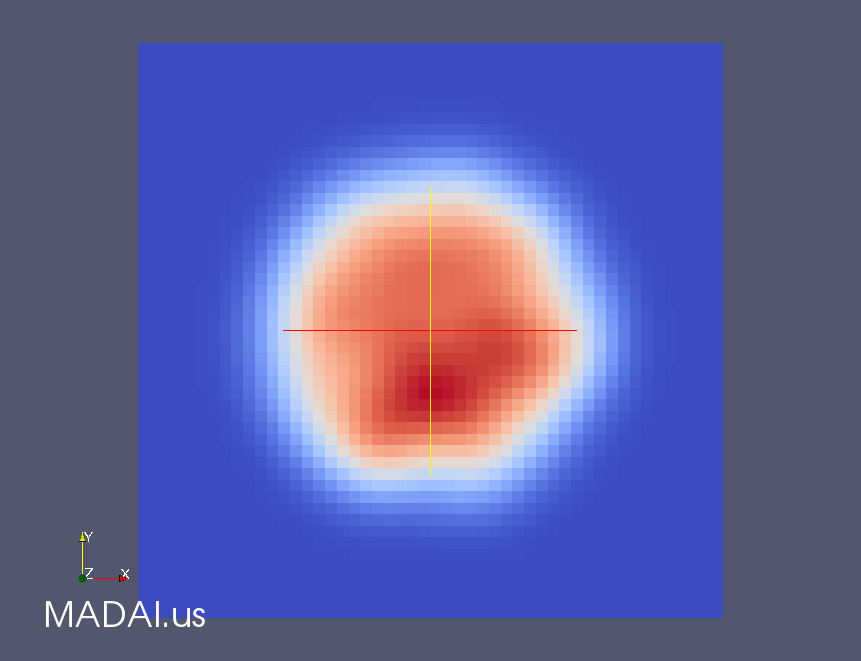
\includegraphics[scale=.22]{images/GaussianScalarSplatterPoint2.png}
   \caption{Point density produced by the \filter{GaussianScalarSplatter} filter (\field{NumberDensity} field) with standard deviation 0.1 (left) and standard deviation 0.2 (right).}
   \label{fig:GaussianScalarSplatter1}
\end{figure}

Now change the \setting{Standard Deviation} value to 0.2 and click \setting{Rescale}. Notice how the splatted result is smoother on the right side of Figure \ref{fig:GaussianScalarSplatter1}.

Finally, color the slice by the \field{X\_Density} field and click the \setting{Rescale} button. Figure \ref{fig:GaussianScalarSplatter2} shows the result.

\begin{figure}[htbp]
   \centering
   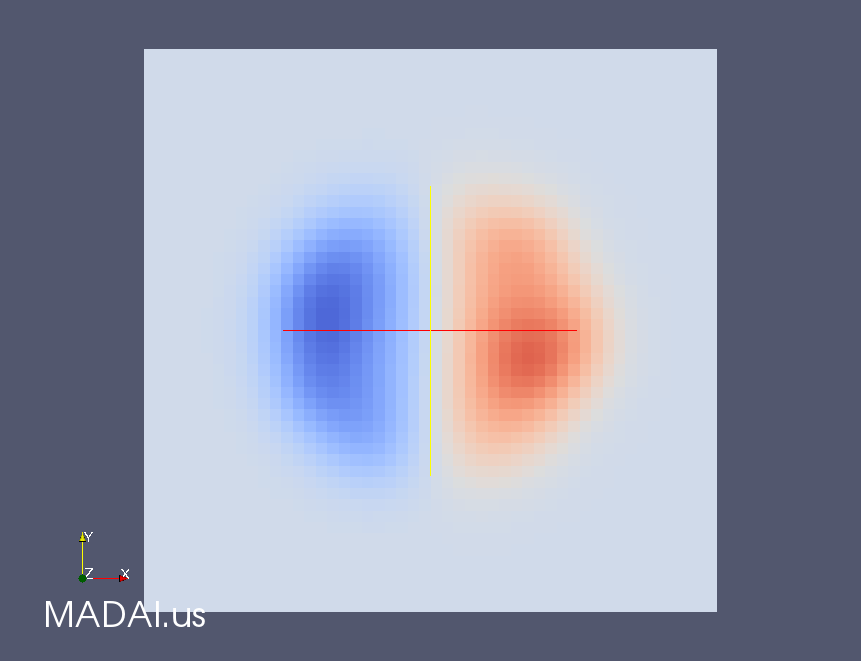
\includegraphics[scale=.25]{images/GaussianScalarSplatterXDensity.png}
   \caption{\texttt{X\_Density} produced by the \filter{Gaussian Scalar Splatter} filter with standard deviation 0.2.}
   \label{fig:GaussianScalarSplatter2}
\end{figure}

\subsection{Ensemble Surface Slicing Representation}

In the ParaView tutorial, we have seen that several representations are available for displaying data in ParaView (\representation{3D Glyphs}, \representation{Outline}, \representation{Points}, \representation{Surface}, \representation{Surface with Edges}, \representation{Wireframe}). Another representation is suitable for displaying a group of surfaces using a technique called Ensemble Surface Slicing \cite{Oluwafemi2012}. In this technique, more than one surface embedded in the same space are all displayed at the same time. However, only slices from each surface are displayed. These slices are interleaved in such a way that the slices from all the surfaces are mostly visible (some slices from one surface may be occluded by slices from other surfaces depending on the shape and viewing angle.

To try this technique, open the files \file{apple.ply}, \file{banana.ply}, \file{cherry.ply}, and \file{grape.ply}. The \representation{Ensemble Surface Slicing} representation operates on a set of surfaces grouped together into what is called a multiblock dataset. A multiblock data set is a hierarchy of other datasets. To group the files, select them all in the pipeline browser by selecting the first file in the browser, then press the shift key and select the last file. Next, group them together with \menu{Filters} $\rightarrow$ \menu{Alphabetical} $\rightarrow$ \menu{Group Datasets}. The resulting display will show the union of the surfaces, the same as what you would get just by having all the surfaces' visibility turned on.

\begin{figure}[htbp]
   \centering
   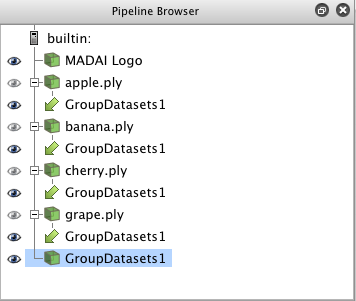
\includegraphics[scale=.5]{images/ESSGroupDatasets.png} % requires the graphicx package
   \caption{The fruit datasets \texttt{apple.ply}, \texttt{banana.ply}, \texttt{cherry.ply}, and \texttt{grape.ply} grouped together.}
   \label{fig:ESSGroupDatasets}
\end{figure}

Next, change the representation of the grouped surfaces to \representation{Ensemble Surface Slicing}. Change the \setting{Slice Width} setting to 2 and the \setting{Plane Normal} to 0, 0, 1. You should see an image similar to Figure \ref{fig:ESSSurfaces}. Each surface is colored by a different color. These colors are automatically chosen to be perceptually well-separated in color space but isoluminant to avoid obscuring the perceived shapes. You can try changing the \setting{Plane Normal} to different values to change the orientation of the slices and the \setting{Slice Width} to change the width of the slices.

\begin{figure}[htbp]
   \centering
   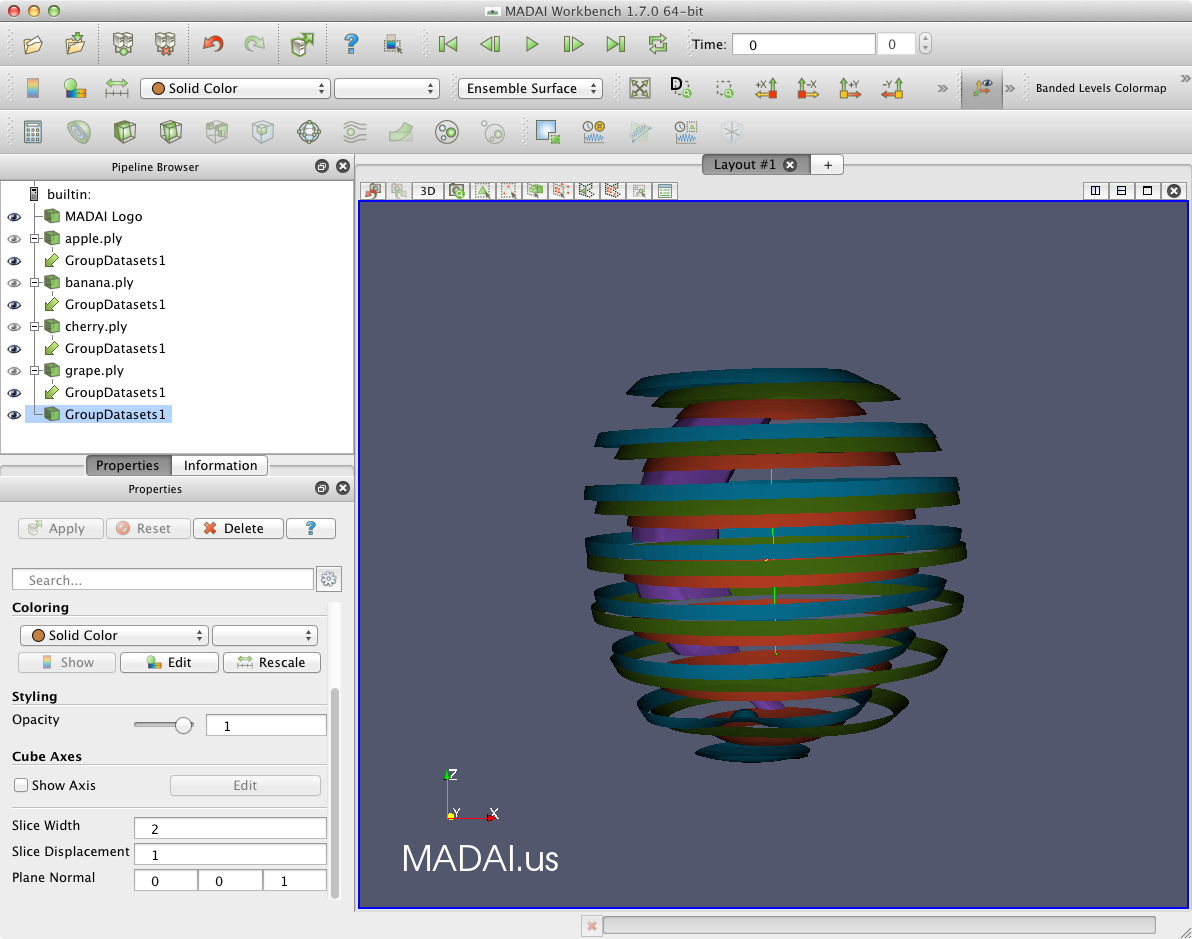
\includegraphics[scale=.25]{images/ESSSurfaces.png} % requires the graphicx package
   \caption{The fruit datasets displayed with the ensemble surface slicing technique.}
   \label{fig:ESSSurfaces}
\end{figure}


\bibliographystyle{plain}
\bibliography{MADAIWorkbenchTutorial}

\end{document}